\chapter{Introduction}

\section{\highlight{Motivation}}

The natural world is rich in visual texture. While a precise definition of 
texture remains to be found, most research consider it as visual patterns that 
exhibit local variations while maintaining global homogeneity, as shown in Fig.\ \ref{fig:texture}.

\begin{figure}[t]
\begin{center}
	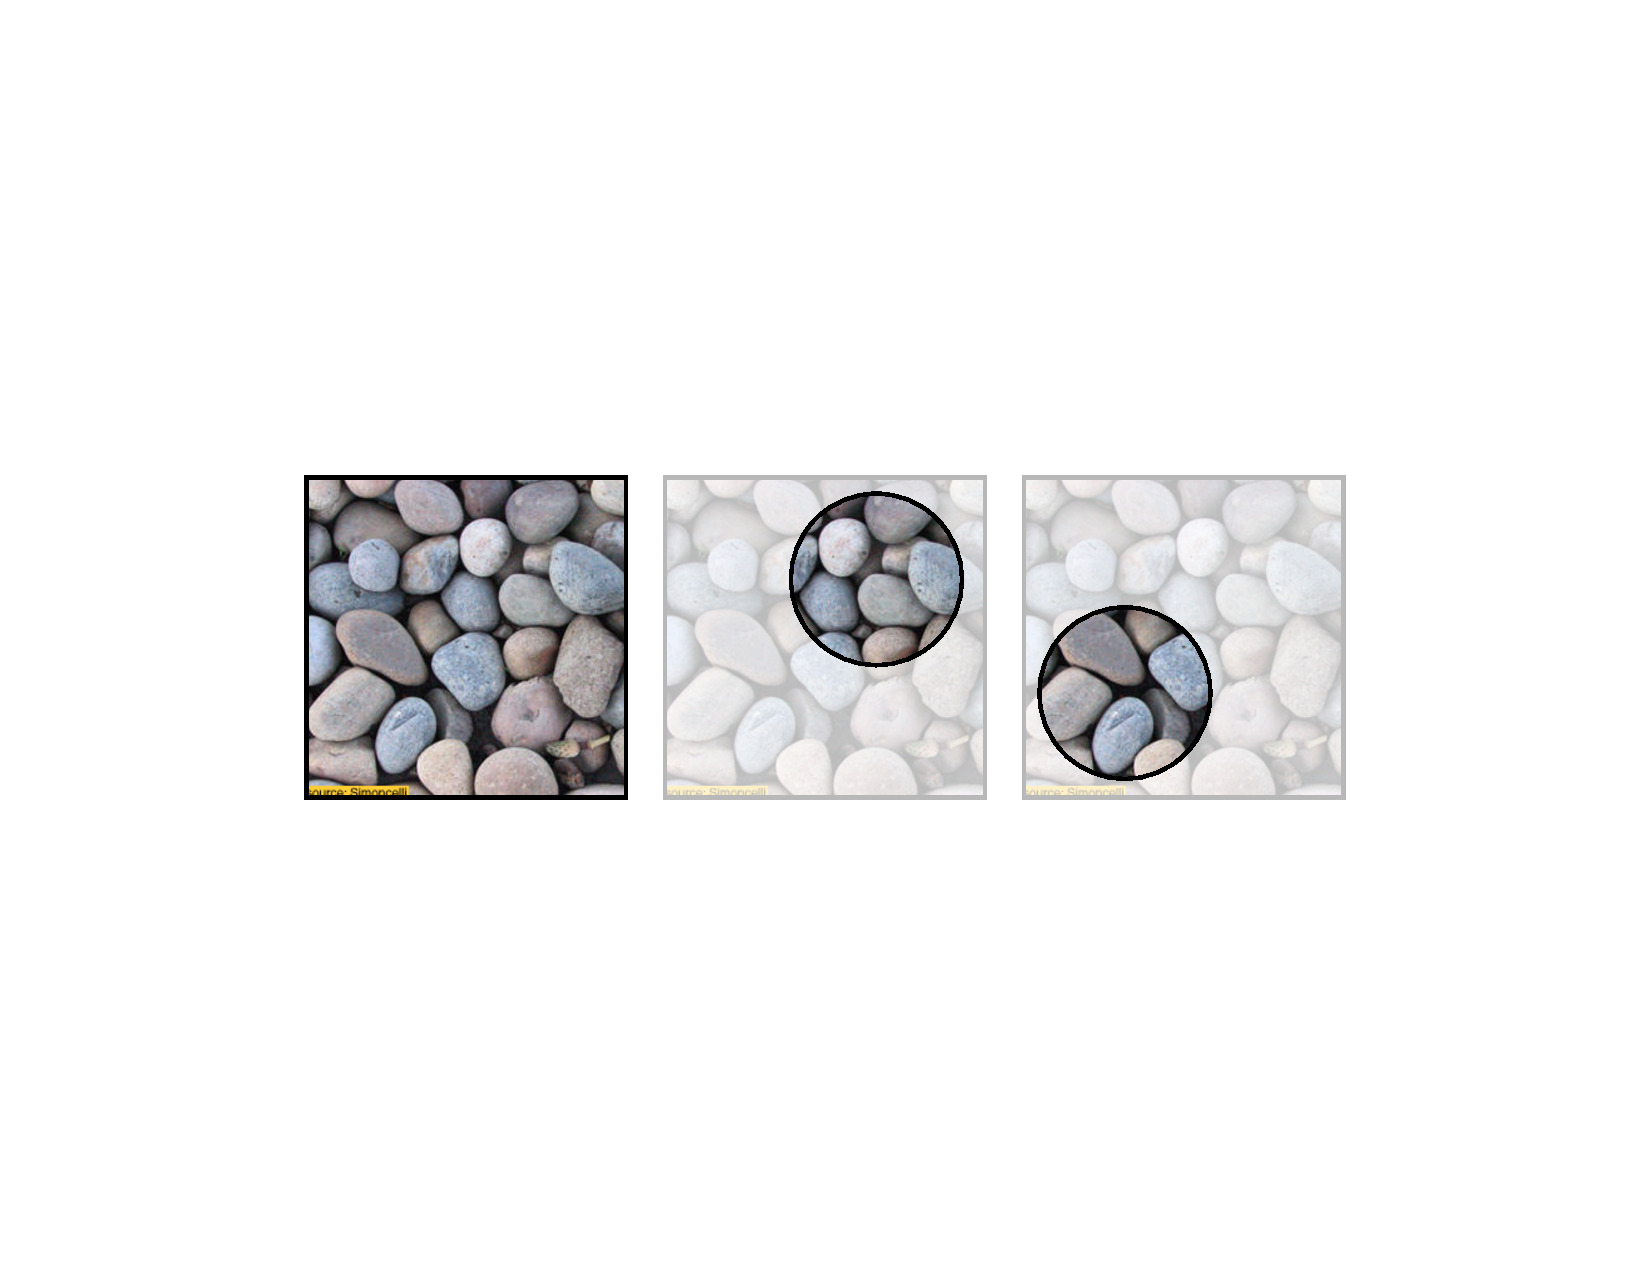
\epsfig{file=texture.pdf, width = 0.8\textwidth}\\
	\caption[Definition of a static texture]{Definition of a static texture. A static texture is a visual pattern that exhibits local spatial variations while maintaining global homogeneity. Observing small apertures across the texture should reveal visual content that appears roughly the same, captured as feature statistics.}
	\vspace{-0.65cm}
	\label{fig:texture}
\end{center}
\end{figure}

Textures 
can be static or dynamic: static textures exist in two-dimensional (2D) image space 
(\eg, grass and water) while dynamic textures extend the notion across time (\eg, 
fluttering grass and wavy water). As a result, local spatial variations and 
global homogeneity extend across space \emph{and} time. These temporal patterns 
have previously been studied under a variety of names, including turbulent flow \cite{heeger1986} (for extracting optical flow from fluids undergoing irregular fluctuations), temporal textures \cite{nelson1992} (for recognition of moving patterns such as windblown trees or rippling water), time-varying 
textures \cite{bar-joseph2001} (for synthesizing stochastically-moving patterns), dynamic textures \cite{doretto2003} (for modelling and synthesizing stochastically-moving patterns), textured 
motion \cite{wang2003} (for modelling and synthesizing patterns undergoing stochastic or consistent motion), and spacetime textures \cite{derpanis2012spacetime} (for classifying dynamic patterns).
In this thesis, the term ``dynamic texture'' is adopted.

Both static and dynamic texture cues play important roles in our perception of 
surfaces. Understanding and characterizing these patterns has long been a problem 
of interest in human perception, computer vision, and computer graphics. In 
computer vision, studying the underlying statistics of textures allows us to gain 
insight as to how these complex structures can be interpreted and how we may be 
able to leverage this knowledge to inform certain vision-related tasks. Examples 
of such tasks include shape-from-texture \cite{gibson1950perception}, \highlight{material recognition \cite{dana1999,adelson2001},} texture 
synthesis \cite{heeger1995pyramid}, and more recently, image style transfer 
\cite{gatys2016image}. In terms of specific applications, 
there are many in the creative-industry including, but not limited to, computer-generated imagery, digital painting, and image editing.

Shape-from-texture involves recovering the
three-dimensional (3D) shape of an object from a 2D image by using texture as a 
cue. Gibson \cite{gibson1950perception} proposed the \emph{texture gradient} as 
the primary basis of surface perception by humans. He conjectured that neighbouring areas on a textured surface are perceived differently only due to differences
in surface orientation and distance from the observer.

\highlight{Material recognition in computer vision involves recognizing material categories (\eg, fabric, water, and wood) from an image based on the visual appearance of surfaces. The visual appearance of a surface depends on several factors \cite{dana1999,adelson2001}, such as illumination, geometric structure at various scales, viewing direction, and surface reflectance properties (\eg, the Bidirectional Reflectance Distribution Function, or BRDF, see \cite{nayar1991}). Notably, texture can be useful for distinguishing materials. For example, wood and water each have unique texture that easily distinguishes the two. Dana \etal \cite{dana1999} introduced the Bidirectional Texture Function (BTF) and demonstrated that the visual appearance of materials can be characterized by measuring texture.}

\begin{figure}[t]
\begin{center}
	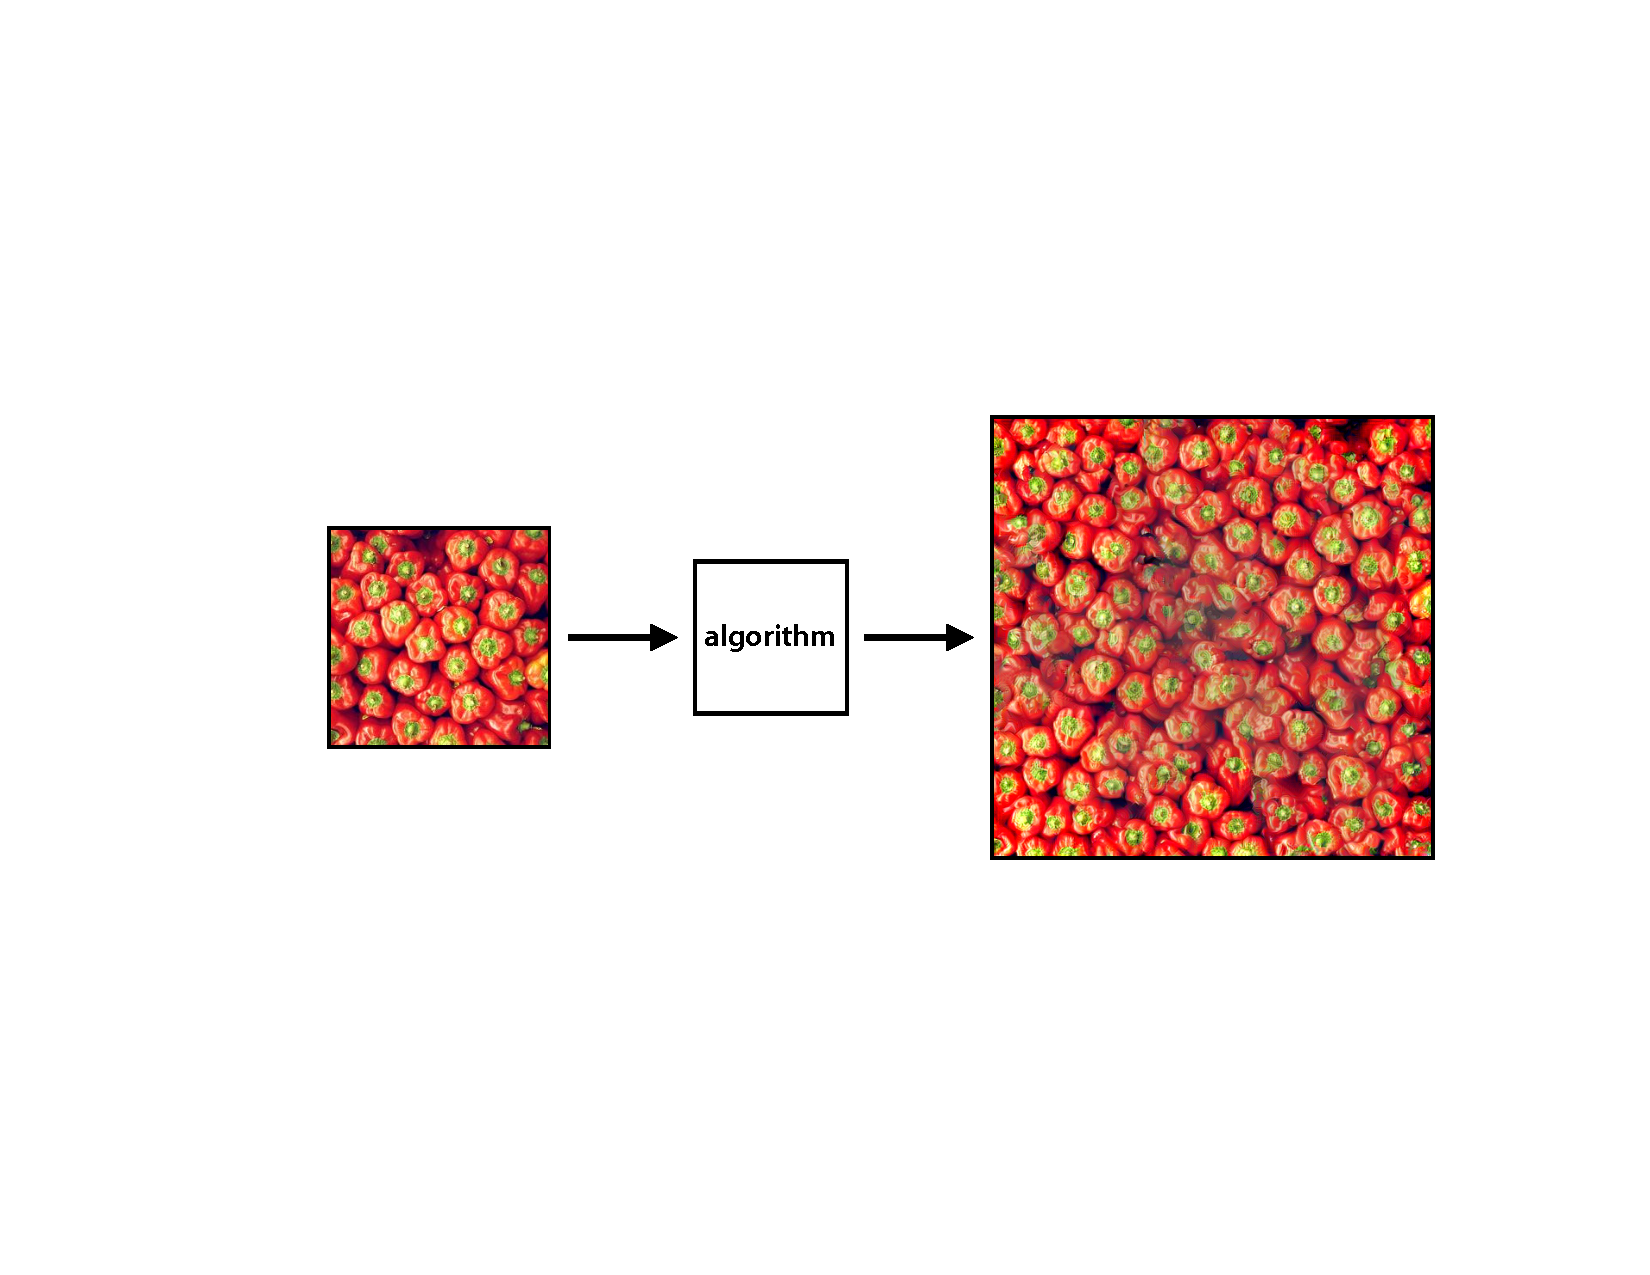
\epsfig{file=texture_synthesis.pdf, width = 0.8\textwidth}\\
	\caption[Texture synthesis.]{(Static) texture synthesis is the process of algorithmically constructing a texture (right) that matches or extends a given source texture (left) by taking advantage of its structural content.}
	\vspace{-0.65cm}
	\label{fig:texture_synthesis}
\end{center}
\end{figure}

Texture synthesis (Fig.\ \ref{fig:texture_synthesis}) is the process of algorithmically constructing a texture that
matches or extends a given source texture by taking advantage of its structural 
content. Heeger and Bergen \cite{heeger1995pyramid} took advantage of the fact 
that two textures are often difficult to discriminate when they produce a similar 
distribution of responses from a bank of linear filters. They used a combination 
of Laplacian and steerable pyramids to deconstruct a given texture and 
synthesized a new texture by matching the distributions of responses from each
pyramid level. Portilla and Simoncelli \cite{portilla2000parametric} extended this approach by including complex ``analytical'' filters that allowed them to utilize measures of local phase and energy in their texture descriptors. More recently, Gatys \etal \cite{gatys2015} demonstrated 
impressive results for texture synthesis by using a convolutional network (ConvNet) instead of a linear 
bank of filters to model the non-linear spatial statistics of a given texture.

\begin{figure}[t]
\begin{center}
	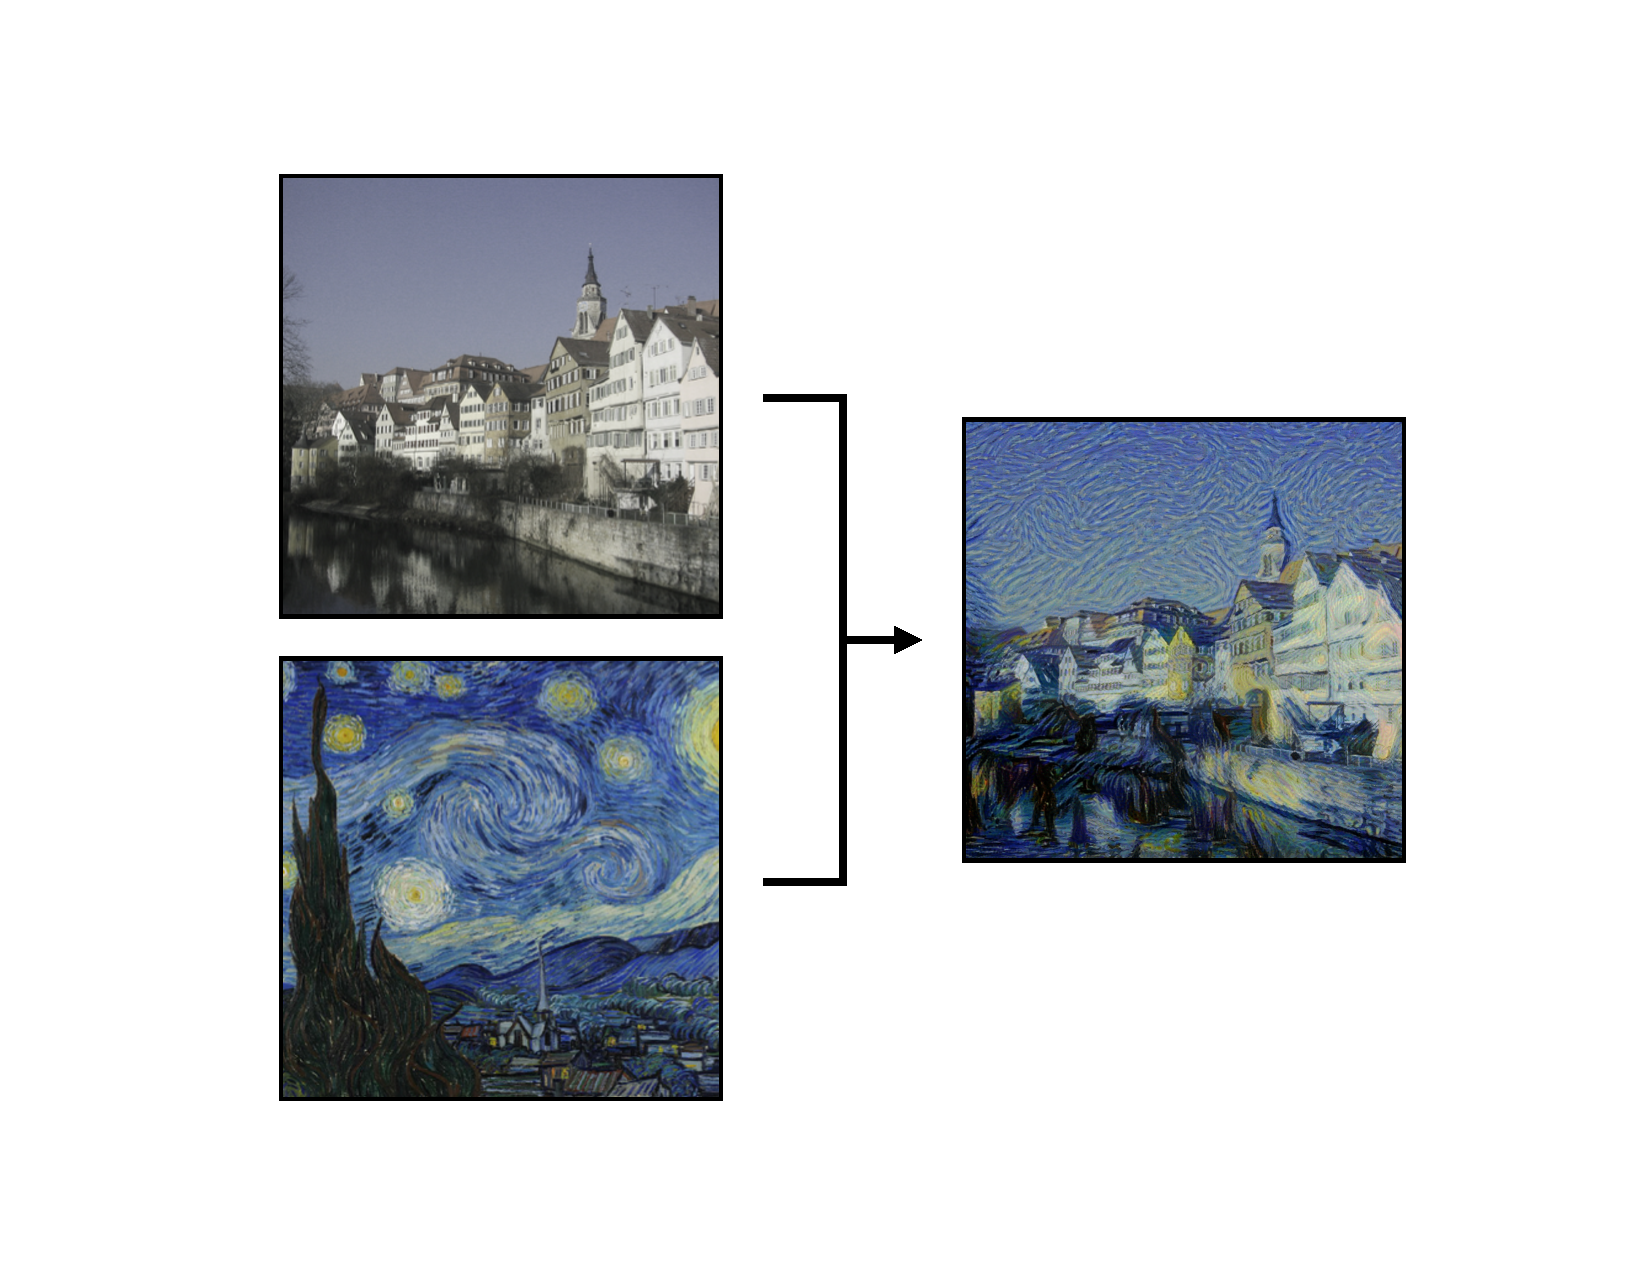
\epsfig{file=style_transfer.pdf, width = 0.6\textwidth}\\
	\caption[Image style transfer]{Image style transfer. The goal is to synthesize a texture (right) from an input ``style'' image (bottom-left) while constraining the process in order to preserve the semantic content of an input ``content'' image (top-left).}
	\vspace{-0.65cm}
	\label{fig:style_transfer}
\end{center}
\end{figure}

Image style transfer (Fig.\ \ref{fig:style_transfer}) is a recent technique where the goal is to 
recompose an image in the ``style'' (\eg, texture) of another image. This can be considered as a 
texture transfer problem, as previously demonstrated by Efros \etal \cite{efros2001image}, where they transferred a given texture to another image by stitching together small patches of the given texture while conforming to the luminance of the other image. Although the simplicity of their approach was attractive, it failed for highly structured textures due to patch boundary inconsistencies, limiting the selection of acceptable textures. 
Gatys \etal \cite{gatys2015} modified their previous ConvNet for texture synthesis to support texture transfer by including an additional objective that enforced the synthesized texture to match the semantic content of a given image, resulting in an image style transfer \cite{gatys2016image}. Unlike the patch-based method of Efros \etal \cite{efros2001image}, Gatys \etal's approach of using a ConvNet was more robust to textures with long-range consistencies.

Motivated by the ConvNet model of Gatys \etal \cite{gatys2015} for texture synthesis, the focus of this thesis is on the synthesis of dynamic texture 
samples, as captured in video, based on a single exemplar through the use of ConvNets. Inspired by Gatys \etal's \cite{gatys2016image} method of image style transfer, a novel form of style transfer for dynamic textures is presented as well.

\section{Summary of thesis}

Many common dynamic textures are naturally described by the ensemble of 
appearance and dynamics (\ie, spatial and temporal pattern variation) of their 
constituent elements. In this thesis, a factored analysis of dynamic 
textures in terms of their appearance and dynamics is proposed.
This factored analysis is then used to enable dynamic texture synthesis
based on an example dynamic texture as input.
It also enables a novel form of style transfer where the 
target appearance and dynamics can be taken from different sources---termed \emph{dynamics style transfer}.
An overview of dynamic texture synthesis and dynamics style transfer
is shown in Fig.\ \ref{fig:teaser}.
\clearpage
\begin{figure}[t]
\begin{center}
	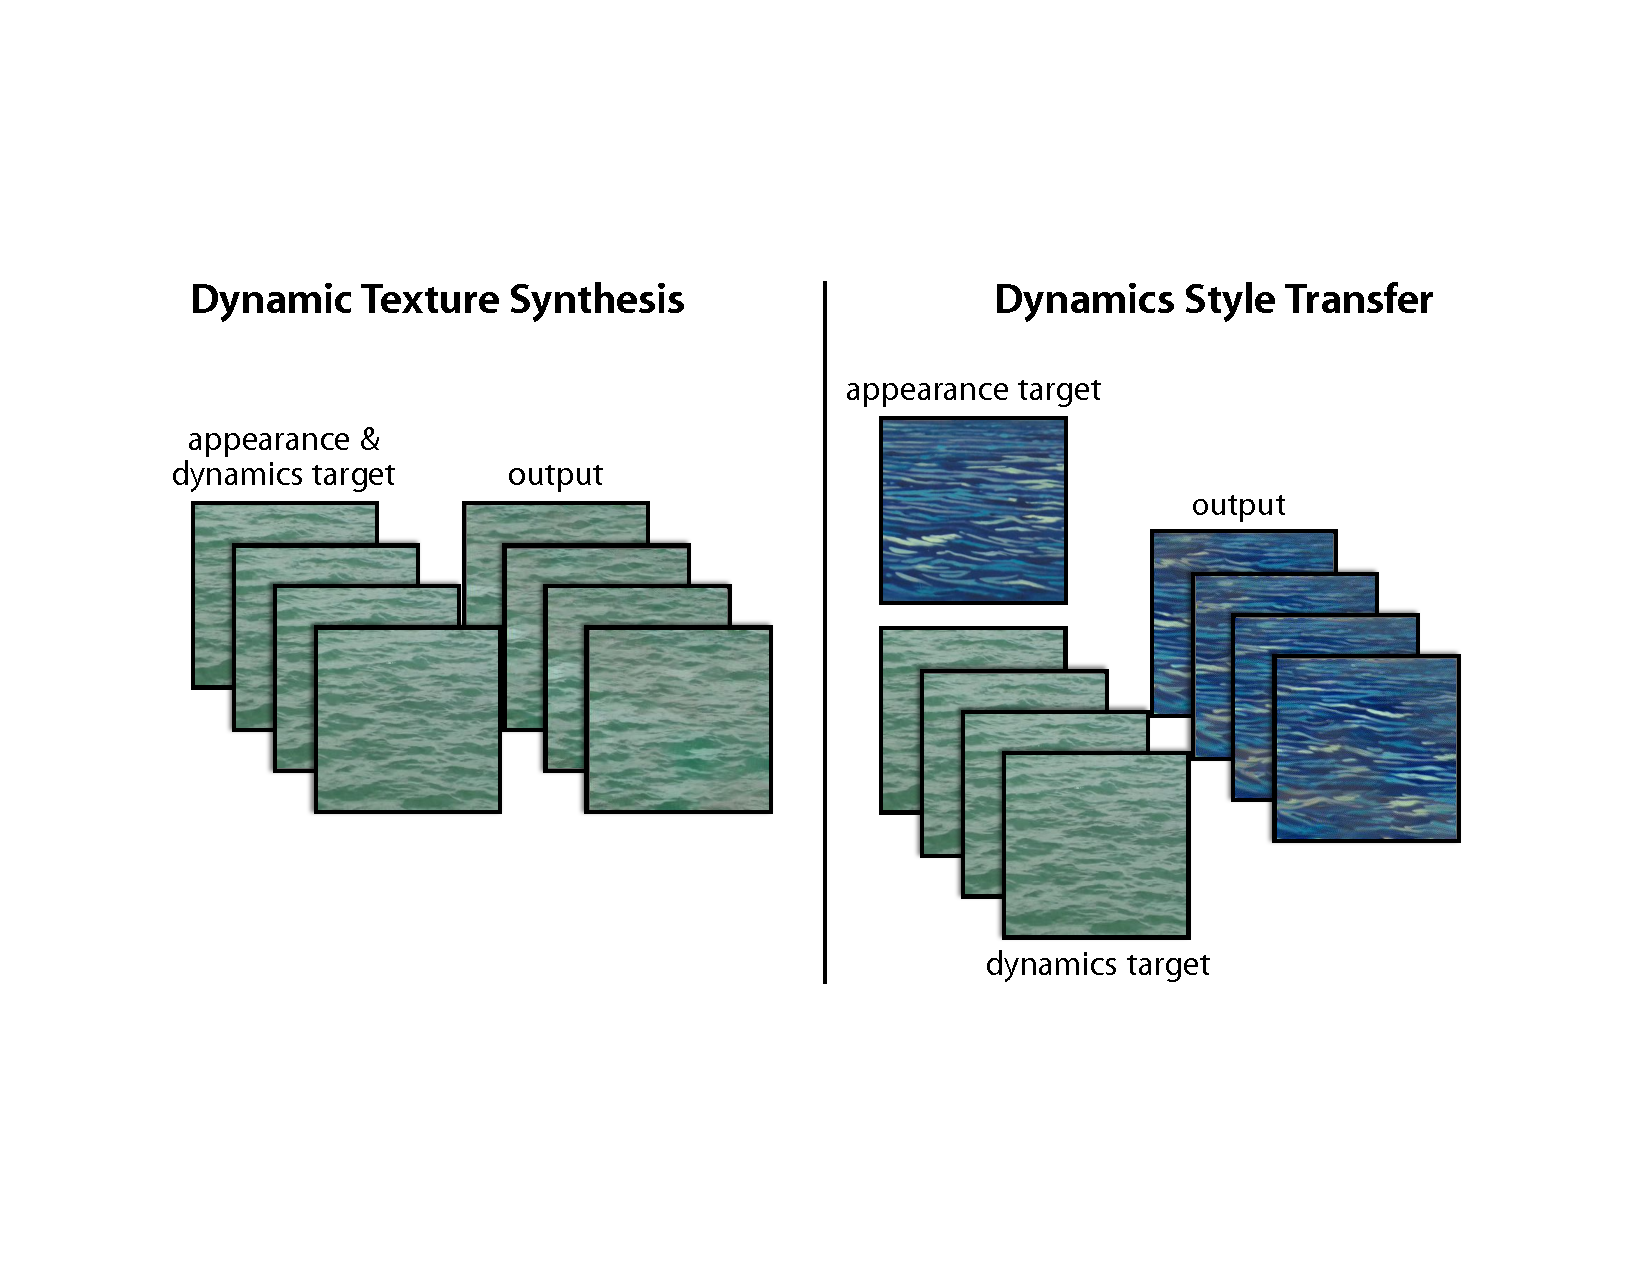
\epsfig{file=teaser.pdf, width = 0.8\textwidth}\\
	\caption[Dynamic texture synthesis.]{Dynamic texture synthesis. (left) Given an input dynamic texture as the target, the two-stream model synthesizes a novel dynamic texture that preserves the target's appearance and dynamics characteristics. (right) The two-stream approach enables synthesis that combines the texture appearance from one target with the dynamics from another, resulting in a composition of the two.}
	\vspace{-0.65cm}
	\label{fig:teaser}
\end{center}
\end{figure}
\clearpage
The proposed model is constructed from two ConvNets: an appearance stream and a dynamics stream,
which have been pre-trained for object recognition
and optical flow \edit{prediction}{estimation}, respectively.
Similar to previous work on spatial textures
\cite{gatys2015,heeger1995pyramid,portilla2000parametric}, an input dynamic texture is summarized in terms of a set of
spatiotemporal statistics of filter outputs from each stream.
The appearance stream models the per-frame appearance of
the input texture, while the dynamics stream models its
temporal dynamics.
The synthesis process consists of optimizing a randomly initialized noise pattern such that its spatiotemporal statistics from
each stream match those of the input texture.
The architecture is inspired by insights from human perception and 
neuroscience.
In particular, psychophysical studies \cite{cutting1982} show that
humans are able to perceive the structure of a dynamic texture even
in the absence of appearance cues, suggesting that the two streams
are effectively independent.
Similarly, the two-stream hypothesis \cite{goodale1992} models the 
human visual cortex in terms of two pathways, the ventral stream
(involved with object recognition) and the
dorsal stream (involved with motion processing). Two-stream networks have also been used for video understanding tasks in computer vision, with particular attention to action recognition \cite{simonyan2014,feichtenhofer2016two}.

In this thesis, the two-stream analysis of
dynamic textures is applied to texture synthesis.
A range of dynamic textures are considered and it is demonstrated that the 
proposed approach generates novel, high quality samples that match
both the frame-wise appearance and temporal evolution of an input
example.
Further, as stated previously, the factorization of appearance and dynamics enables a 
novel form of style transfer, where the dynamics of one texture are 
combined with the appearance of a different one,
\cf\ \cite{gatys2016image}.
This can even be done using a single image as an appearance
target, which allows static images to be animated.
Finally, the perceived realism of the generated textures is validated
through an extensive user study.

\section{Contributions}

The contributions of this work span both theory and application. Specifically, this thesis presents the key components for creating the proposed dynamic texture synthesis model, resulting in four primary contributions to the dynamic texture literature.

\begin{enumerate}
	\item \textbf{Factored representation of appearance and dynamics}. First, theoretical insight into the characterization of dynamic textures is provided by building a novel factored representation of both appearance and dynamics. Qualitatively, the two-stream representation is effective in generating visually compelling, novel instances of a wide range of dynamic textures.
	\item \textbf{Motion energy representation of dynamics via a ConvNet}. Second, for the representation of dynamics, a novel ConvNet based on a ``marginalized'' motion energy model \cite{derpanis2010role,derpanis2012spacetime} is constructed and trained on the proxy task of optical flow prediction. This representation of dynamics provides a substantial improvement to the quality of synthesized textures when compared to using optical flow directly.
	\item \textbf{Dynamics style transfer}. Third, a novel form of style transfer is demonstrated, where the dynamics of a dynamic texture can be mixed with the spatial appearance of a different (static or dynamic) texture. This is enabled by the proposed factored representation.
	\item \textbf{Quantitative evaluation via user study}. Finally, a quantitative evaluation on the limitations of the method is performed through the inclusion of a broad range of textures and an extensive user study. This analysis \edit{will provide}{provides} insight for the types of characteristics of temporal imagery that may cause a breakdown of the proposed model. \edit{This}{These insights} may point to future work to address limitations of the proposed model.
\end{enumerate}